%*----------- SLIDE -------------------------------------------------------------
\begin{frame}[t]{Educação}
    A pandemia de COVID-19 representou não somente uma crise
    sanitária de proporções históricas, como resultou na maior adversidade, até então, enfrentada pela educação básica brasileira.
    \newline
    %\vspace{0.5cm}
    \begin{table}[ht!]
    \centering
        \begin{center}
            \begin{figure}
                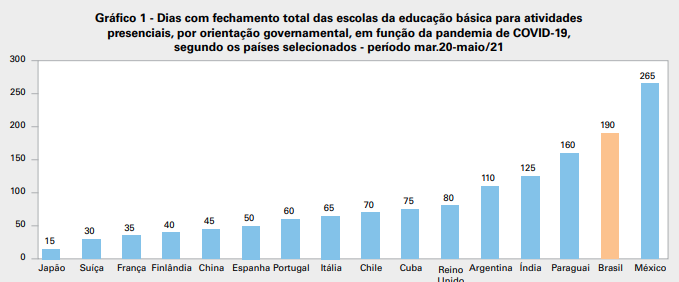
\includegraphics[width=.75\textwidth]{educação1.png}          
            \end{figure}
        \end{center}
    \end{table}
%*----------- notes
    \note[item]{Notes can help you to remember important information. Turn on the notes option.}
\end{frame}
%-
%*----------- SLIDE -------------------------------------------------------------
\begin{frame}[t]{Educação}
    
    \begin{table}[ht!]
    \centering
        \begin{center}
            \begin{figure}
                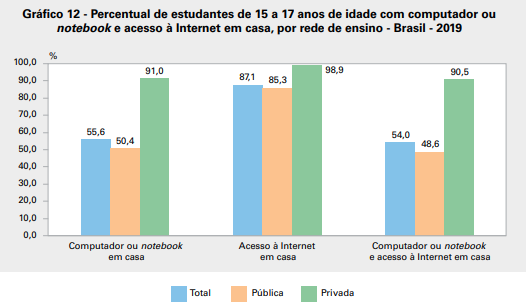
\includegraphics[width=.75\textwidth]{educação2.png}          
            \end{figure}
        \end{center}
    \end{table}
    %\vspace{0.5cm}
    % \begin{table}[ht!]
    % \centering
    %     \caption{PERCENTUAL DE CONCLUSÃO POR EQUIPE}
    %     \begin{tabular}{|l|c|c|c|c|} \hline
    %         \textbf{EQUIPE}&\textbf{04/05}&\textbf{11/05}&\textbf{18/05}&\textbf{25/05}\\ \hline
    %         RAJA & 17\% &32\% & &  \\ \hline
    %         BORG & 0\% &41\% & &  \\ \hline
    %         TIMON-HM & 5\% &47\% & &  \\ \hline
    %     \end{tabular}
    % \end{table}
%*----------- notes
    \note[item]{Notes can help you to remember important information. Turn on the notes option.}
\end{frame}
%-